\documentclass{standalone}
\usepackage{tikz}
\usepackage{ctex,siunitx}
\setCJKmainfont{Noto Serif CJK SC}
\usepackage{tkz-euclide}
\usepackage{amsmath}
\usetikzlibrary{patterns, calc,3d}
\usetikzlibrary {decorations.pathmorphing,decorations.pathreplacing,decorations.shapes}
\begin{document}
\small
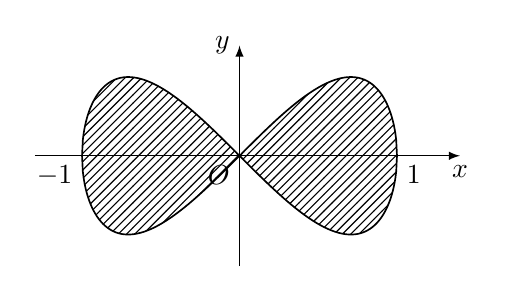
\begin{tikzpicture}[>=latex,scale=2.0]
  \draw[->](-1.3,0)--(1.4,0)node[below]{$x$};
  \draw[->](0,-0.7)--(0,0.7)node[left]{$y$};
  \draw[samples=200,domain=-1:0,semithick,pattern=north east lines ]plot(\x,{sqrt(\x*\x-\x*\x*\x*\x)});
  \draw[samples=200,domain=-1:0,semithick,pattern=north east lines ]plot(\x,{-sqrt(\x*\x-\x*\x*\x*\x)});
  \draw[samples=200,domain=1:0,semithick,pattern=north east lines ]plot(\x,{sqrt(\x*\x-\x*\x*\x*\x)});
  \draw[samples=200,domain=1:0,semithick,pattern=north east lines ]plot(\x,{-sqrt(\x*\x-\x*\x*\x*\x)});
  \node at (-1,0)[below left]{$-1$};
  \node at (1,0)[below right]{$1$};
  \node at (0,0)[below left]{$O$};
\end{tikzpicture}
\end{document}